\documentclass[10pt,a4paper]{article}
\usepackage[utf8]{inputenc}
\usepackage{amsmath, amsfonts, amssymb, amsthm}
\usepackage{mathtools, array, enumitem, xcolor}
\usepackage[margin=0.7in]{geometry}
\setlength{\parindent}{0em}

\usepackage[czech]{babel}

\theoremstyle{plain}
\newtheorem{veta}{Věta}
\theoremstyle{definition}
\newtheorem{definice}[veta]{Definice}


\title{Řešení domácího úkolu z MA č. 13}
\author{přezdívka: Zdeněk}
\date{}

\begin{document}

\maketitle

\section{}


\begin{enumerate}[label=(\alph*)]

\item 

\[ \int_0^4 \frac{dx}{1+\sqrt{x}} \]

\[ y = \sqrt{x}\]
\[ \frac{dy}{dx} =\frac{1}{2\sqrt{x}} = \frac1{2y} \implies dx =  dy 2y \]

\[ = 2 \int_0^2 \frac{y}{1+y} dy = 2 \int_0^2 1 - \frac{1}{1+y} dy  = 2 [x]_0^2 - 2[\ln(1+x)]_0^2 \]
\[ = 4 - 2 \ln(3) = 4 - \ln(9) \approx 2\]

\item

\[ \int_0^{\frac{\pi}{3}} \frac{\tan(x) }{1 + \cos^2(x) } dx  \]


\[
\int_0^{\frac{\pi}{3}} \frac{\tan(x) }{1 + \cos^2(x)} dx
\]

\[ y = \cos(x) \]
\[ \frac{dy}{dx} = - \sin(x) \implies dx = -\frac{dy}{\sin x}\]

\[
= \int_1^{\frac12} - \frac{1}{y(1 + y^2)} dy
\]

\[ z = y^2 \]
\[\frac{dz}{dy} = 2y \implies dy = \frac{dz}{2y}  \]


\[
= \int_1^{\frac14} - \frac12 \frac{1}{z(1 + z)} dz
= \frac12 \int_{\frac14}^1  \frac{1}{z(1 + z)} dz
= \frac12 \int_{\frac14}^1  \frac{1}{1 + z} - \frac{1}{z} 
= \frac12 [ln(x+1) - ln(x)]_{\frac14}^1 \]\[
=\frac12 [ln(1+x^-1)]_{\frac14}^1 
= = \frac12 \left( \ln(5) - \ln(2) \right) = \frac12 \ln\left( \frac52 \right)
\]

\section{Torus}

\begin{figure}[hbtp]

\centering
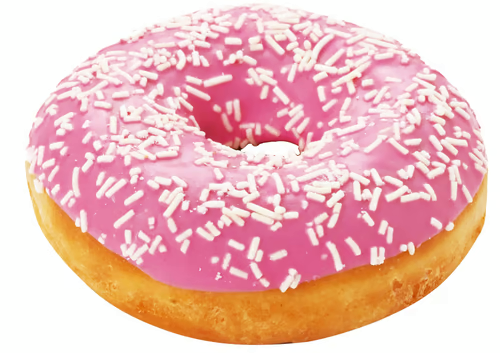
\includegraphics[scale=0.2]{torus.png}
\caption{Torus}
\end{figure}


\begin{enumerate}
\item Využijeme vztah pro objem rotačního tělesa
\[ V = \int_a^b \pi f^2(x) d x \]

Jako $f$ použijeme kružnici $k([0, R], r)$, rozdělenou na dvě části:

\[x^2 + y^2 = r^2 \implies y = \pm \sqrt{r^2 - x^2}\]
\[ f_1(x) = \sqrt{r^2 - x^2} + R \]
\[ f_2(x) = -\sqrt{r^2 - x^2} + R \]

\[ V = \int_{-r}^{r} \pi \left(\sqrt{r^2 - x^2} + R \right)^2 d x - \int_{-r}^{r} \pi\left(-\sqrt{r^2 - x^2} + R \right)^2 d x \]

\hfill

\[ \left(\sqrt{r^2 - x^2} - R \right)^2 - \left(-\sqrt{r^2 - x^2} + R \right)^2 =  4R\sqrt{r^2-x^2}  \]

\[ V = \int_{-r}^{r} \pi 4R\sqrt{r^2 - x^2}  d x 
	= 4 \pi R \int_{-r}^{r} \sqrt{r^2 - x^2} d x 
\]

Tento integrál jsme již řešili pomocí substituce $x = ry$ a následné substituce $y = cos u$. Nebo taky můžeme ověřit Wolframem.
	
\[  \overset{Wolfram}{=} 4 \pi R \frac12 \pi r^2 = 2 \pi^2 R r^2
\]

\item Využijeme vztah pro objem rotačního tělesa
\[ S = \int_a^b 2\pi f(x) \sqrt{1 + \left( \frac{df(x)}{dx}\right)^2} d x \] 

Tentokrát povrchy daných těles sečteme.

 \[ \frac{d(\pm \sqrt{r^2 - x^2} + R)}{dx} \overset{Wolfram}{=} \mp \frac{x}{ \sqrt{r^2 - x^2}} \]
 \[ \left( \pm \frac{x}{ \sqrt{r^2 - x^2}} \right)^2 = \frac{x^2}{r^2-x^2} = - \frac{x^2 - r^2 + r^2}{x^2 - r^2} = - 1 + \frac{r^2}{ r^2 - x^2}\]
 
 Jedinčky pod odmocninou se odečtou.
 
 \[ S_1 = \int_{-r}^{r} 2\pi \left(\sqrt{r^2 - x^2} + R\right)  \sqrt{1 + - 1 + \frac{r^2}{x^2 - r^2}} d x
     = \int_{-r}^{r} 2\pi \left(\sqrt{r^2 - x^2} + R\right)  \frac{r}{\sqrt{r^2 - x^2}} d x    
  \] \[
 =  2\pi r \int_{-r}^{r} 1 + \frac{R}{\sqrt{r^2 - x^2}}   d x    
  \]
 
 
  \[ S_2 = \int_{-r}^{r} 2\pi \left(-\sqrt{r^2 - x^2} + R\right)  \sqrt{1 + - 1 + \frac{r^2}{r^2 - x^2}} d x\] \[
 =  2\pi r \int_{-r}^{r} -1 + \frac{R}{\sqrt{r^2 - x^2}}   d x    
  \]
  
  
\hfill

Jedničky se odečtou. 


\[ S_1 + S_2 = 2\pi r  \int_{-r}^{r}  2 \frac{R}{\sqrt{r^2 - x^2}} 
= 4\pi r R  \int_{-r}^{r} \frac{1}{\sqrt{r^2 - x^2}} \]

\[  \int_{-r}^{r} \frac{1}{\sqrt{r^2 - x^2}} \overset{Wolfram}{=} \pi \]

\[ S = 4\pi^2 r R\]
 

\end{enumerate}




\end{enumerate}

\end{document}